\documentclass{standalone}

\usepackage[compat=1.1.0]{tikz-feynman}

\begin{document}

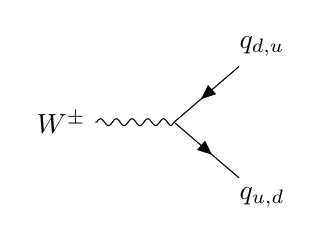
\begin{tikzpicture}
\begin{feynman} [small]
	\vertex (g);
    \vertex [left=of g] (a1) {\(W^\pm\)};
    \vertex [above right=of g] (a2) {\(q_{d,u}\)};
	\vertex [below right=of g] (a3) {\(q_{u,d}\)};
    \diagram* {
    (a1) -- [boson] (g), 
    (a2) -- [fermion] (g), 
    (g) -- [fermion] (a3), 

    };

\end{feynman}
\end{tikzpicture}

\end{document}
